\documentclass{paper}
\usepackage{times}
\usepackage{geometry}
\geometry{letterpaper, portrait, margin=1in}
\usepackage{setspace} \doublespacing
\usepackage[utf8]{inputenc}
\usepackage{enumitem,amssymb}
\usepackage{ragged2e}
\usepackage{physics}
\usepackage{siunitx}
\sisetup{separate-uncertainty=true}
\usepackage{float}

\usepackage{caption}
\usepackage[hidelinks]{hyperref}
\usepackage{url}

\usepackage{graphicx}
\usepackage{epstopdf}
\usepackage{tikz}
\graphicspath{{data/concepts}}

\usepackage{aas_macros}
\usepackage[style=authoryear]{biblatex}
\bibliography{refs} %refs.bib
\nocite{*}

\immediate\write18{texcount \jobname.tex -out=\jobname.sum}

% set frameboxes to be borderless
\setlength{\fboxsep}{0pt}
\setlength{\fboxrule}{0pt}

\begin{document} 

\title{The constituents of the universe and the growth of structure}
\author{ariahayd}
\date{April 24, 2022}
\maketitle

% Overview. [8]
% Give an overview of the current standard model for the context of the essay. 
% Include one figure for this section. 
\section{Overview}
  The universe is shaped by its constituent energies, and its constituents are
  shaped by the size and structures of universe. The densities of energy in
  the fields within the universe determine the geometry of space. The extent
  of space determines how structures evolve over the history of the universe.

  The evolution of the universe is understood through the Standard Model of 
  Cosmology, developed mainly over the last century of observations of matter 
  and energy on large scales, of galaxies and throughout \(Gpc^3\) volumes 
  space, and on the very small scales where the quantum mechanical properties 
  of energy fields emerge. 

  Today's most successful model is called \(\Lambda CDM\), with dynamics 
  dominated by what can be explained through General Relativity, Quantum Field 
  Theory, and with contributions from Dark Energy (\(\Lambda\)) and Cold Dark 
  Matter (\(CDM\)). These last two components are observationally confirmed 
  but not entirely explained by theory. In this model, the metric of the 
  universe is flat \(k=0\), and the equation of parameter \(w\), is constant 
  in time.

  Constraining the free parameters of the physics of the Standard Model to
  fit the best observations of the universe today produces a benchmark model,
  which can be broken down into contributions of different 
  constituents to the energy density of the unverse in the following way,
  (\cite{ryden2003introduction}):

  \begin{center}
  \begin{tabular}{ c c c }
    Photons & \(\Omega_{\gamma} = 5.35E-5 \) \\
    Neutrinos & \(\Omega_{\nu} = 3.65E-5 \) \\
    Total radiation & \(\Omega_{r} = 9.0E-5 \) \\
    Baryonic matter & \(\Omega_{b} = 0.048 \) \\
    Nonbaryonic matter & \(\Omega_{dm} = 0.262 \) \\
    Total matter & \(\Omega_{m} = 0.31 \) \\
    Cosmological constant & \(\Omega_{\Lambda} \approx 0.69 \)
 \end{tabular}
 \end{center}

% 2. Dark Matter. [20]
% Describe two lines of evidence for dark matter. These should be distinct and 
% complementary. A line of evidence can consist of more than one observational 
% phenomenon that together provide the evidence. Include two figures for this 
% section.
\section{Dark Matter}
  Large, gravitationally bound systems such as galaxies and galaxy clusters 
  appear to be embedded in gravitational potentials deeper than expected given 
  the observable masses interacting within the system. The depth of these 
  potentials is inferred to be due to unobserved, \textit{dark} matter.

  % line of evidence one
  Early evidence for Dark Matter in the halo of a galaxy comes from
  measurements of the rotational velocities of the material in the arms of
  spiral galaxies. A spiral galaxy is a stable, virialized structure bound by
  gravity and is expected to follow the Newtonian gravitation model for a
  fluid rotating around a center mass. The spiral arms are not coherent
  structures in themselves, but are the result of a density way propagating 
  through the fluid hydrodynamics of the galactic disk. 

  The rotational velocity of the disk can be estimated via the 
  width of the HII emission lines across the disk of the galaxy, as was done
  for M31 (\cite{1970ApJ...159..379R}), showing the velocity field follows a 
  profile more like a solid body rotating around a center mass than a fluid 
  swirling around a core. Because the dynamics of galaxies can indeed be 
  modeled as a fluid, the only explanation for a velocity field continuing 
  beyond the visible matter of the galaxy is for an unobservable mass 
  encircling the galaxy in a spherical halo.

  \begin{figure}[!htb]
    \begin{centering}
    \includegraphics[scale=0.4]{DM-masscurve.pdf}
    \caption{Fourteen different mass models fitting the velocity map data of
      M31 are combined to yield a band of mass estimates, on the left, and 
      surface densities, on the right, from the center to beyond the luminous 
      edge of M31, a galaxy considered to have an has an apparent angular 
      diameter of \SI{178}{arcsec}.
    Credit: Rubin et al. 1970}
    \label{fig:DM-masscurve}
    \end{centering}
  \end{figure}

  %line of evidence two
  That Dark Matter could not be contributed entirely by baryonic particles
  has been clear since the 1980s. (\cite{liddle2015introduction})

  The modeled energy density of the universe is greater than the mass density
  component due to baryons and radiation alone. 
  (\cite{Clowe_2006})

  Explanations of Dark Matter can be categorized two ways; either due to 
  massive, compact halo objects (MACHOs) or by weakly interacting massive 
  particles (WIMPs). Searches for MACHOs, large, bound bodies in a galatic 
  halo, have returned no significant findings. Though Dark Matter can be 
  observed through phenomena understood through the standard model, there is 
  no candidate WIMP particle that could constitute Dark Matter in the standard 
  model. An explanation of the WIMP contribution to Dark Matter as something 
  like a primordial, massive graviton, requires new physics.
  (\cite{PhysRevLett.128.081806})

% 3. Baryons. [20]
% Describe one indirect constraint on the baryon density (BBN or CMB), and key 
% direct measurements of various baryonic components. Include two figures for 
% this section.
\section{Baryons}
  Constraints on the density of baryons among the matter of the universe are
  based on modeling the prevalence of atoms generated during the big bang 
  nucleosynthesis era or of by modeling angular size of harmonic patterns of
  density waves oscillating through the baryon-photon fluid at the time of
  decoupling. Both approaches for constraining the baryonic contribution
  to the matter density are indirect because the methodologies infer the 
  baryonic prevalence from understood physics at early times rather than
  from direct measurements.

  That primordial chemical elements would have been produced in the 
  environment of a hot big bang, and that the duration of expansion rather 
  than temperature would determine the prevalence of elements, was theorized 
  (\cite{PhysRev.73.803}) before the term ''big bang'' was coined 
  (\cite{Hoyle1949}) and well before the debate over a big bang or continuous 
  creation origin had been decided.

  Big bang nucleosynthesis occurred early in the 

  \begin{figure}[!htb]
    \begin{centering}
    \includegraphics[scale=0.4]{BBN-ratios.pdf}
    \caption{A modeled prediction of the abundances of nuclei through Big
      Bang Nucleosynthesis.
    Credit: Liddle 2015}
    \label{fig:DE-ratios}
    \end{centering}
  \end{figure}


  Measuring the metal content of stars as ''chronometers'' in the least active 
  globular clusters, which are assumed to be the best preserved early 
  environments that can be observed nearby, indicates an age of the universe
  of 15.6+4.6 Gyr. %TODO fix this units
  (\cite{1999ApJ...521..194C})

% 4. Dark Energy. [20]
% Describe two lines of evidence for dark energy. Comment on possible 
% modifications to the standard model. Include two figures for this section.
\section{Dark Energy}
  The energy density of the universe seems to be driven to the critical 
  density that results in flat spatial metric, even at points in the
  the standard model evolution of the universe in which it could be expected
  to deviate away from the critical density due to the geometric shaping 
  effects of matter and radiation energy density.

  The pressure nudging spacetime to a flat curvature in the current epoch is 
  known as Dark Energy, the \(\Lambda\) component of the \(\Lambda CDM\)
  model, because the source of energy has not yet been fully explained, 
  however, it is latent energy density of the vacuum of spacetime in a phase
  greater than a possible groundstate.

  Evidence for Dark Energy in the \(\Lambda CDM\) model comes from two major
  observations that independently constrain the contribution of \(\Lambda\) 
  to the energy budget, measurements of the recession of supernovae as 
  standard candles and measurements of the angular size of standard rulers in 
  the cosmic microwave background anisotropy.

  Fig. \ref{fig:DE-sn_lightcurve} is a Hubble diagram showing the redshift in
  spectrum of surveyed supernovae events. Assuming redshift to be a proxy for
  recession velocity, the data indicate that an increase in recession 
  velocity with distance from the observer, implying an acceleration between
  the positions of observation and event against the rest frame of a
  fundamental observer.

  % supernovae \cite{Riess_1998}
  \begin{figure}[!htb]
    \begin{centering}
    \includegraphics[scale=0.4]{DE-sn_lightcurve.pdf}
    \caption{The figure on the top is a fit of a measurement of the multicolor 
      light curve shape (MLCS) characteristic of SNe Ia as a function of 
      measured redshift of the event spectrum. The figure below is the
      difference between measured magnitude and modeled magntiude for an 
      environment with no Dark Energy, i.e. \(\Omega_{\Lambda} = 0\), to show
      that observations convincingly deviate from an \(\Omega_{\Lambda} = 0\) 
      environment.
    Credit: Riess et al. 1998}
    \label{fig:DE-sn_lightcurve}
    \end{centering}
  \end{figure}


  The Supernova Cosmology Project, completed in 2011, added ten more supernova 
  events to the Hubble diagram \cite{2012ApJ...746...85S}.
  \begin{figure}[!htb]
    \begin{centering}
    \includegraphics[scale=0.4]{DE-constraints.pdf}
    \caption{Constraints on the free parameters of the \(\Lambda CDM\)
      model predicting a range of values for \(\Omega_{m}\) and 
      \(\Omega_{\Lambda}\). The topographic lines of each parameter represent 
      confidence intervals in the measurement. This figure excludes systematic
      errors in the supernovae measurements.
    Credit: Suzuki et al. 2011}
    \label{fig:DE-constraints}
    \end{centering}
  \end{figure}

% 5. Growth of structure. [24]
% Describe how initial fluctuations from inflation have grown to form galaxies. 
% Consider the growth rate on various scales, and the different behaviour of 
% dark matter and baryons.  Include two figures for this section. 
\section{Growth of Structure}

%behavior of dark matter halos accreting baryonic test particles
  Fig. \ref{fig:Struct-halo_accretion} is a simulation of %TODO finish this
  (\cite{2005Natur.435..629S})

  \begin{figure}[!htb]
    \begin{centering}
    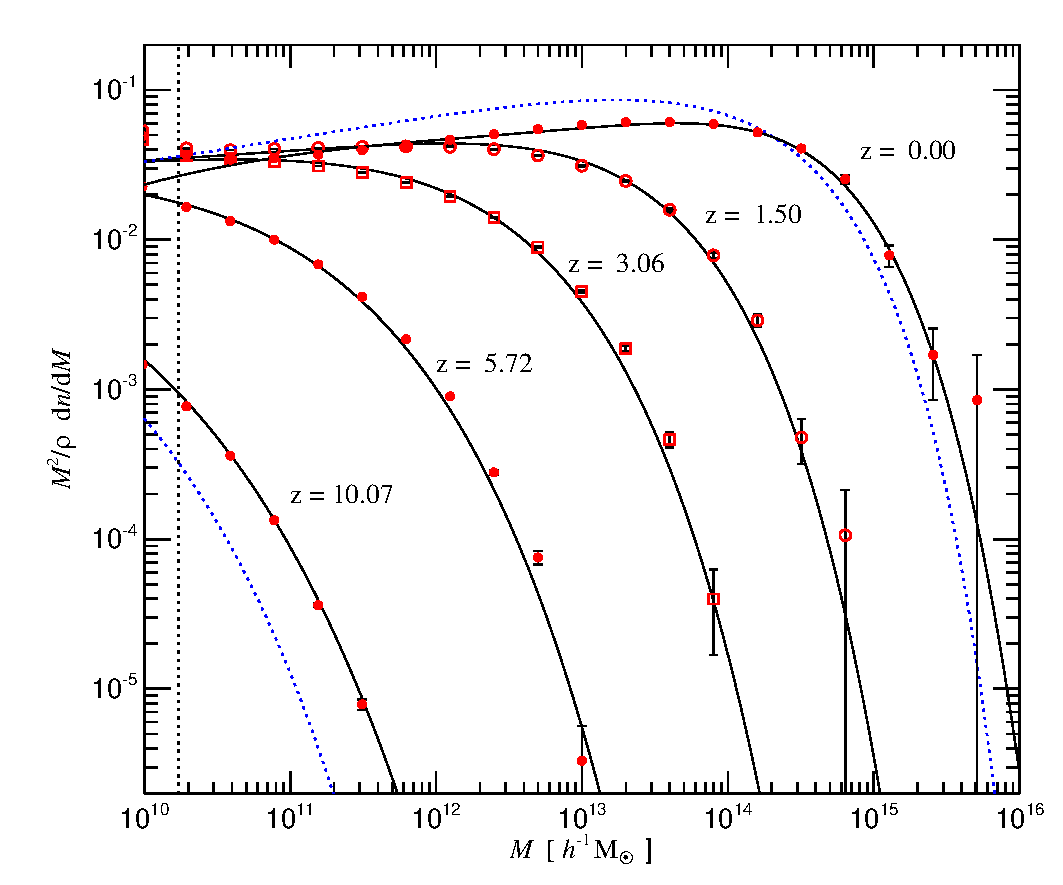
\includegraphics[scale=0.6]{Struct-halo_accretion.pdf}
    \caption{The Millennium Simulation generated number density of halos of 
      baryonic test particles accreting into Dark Matter halos for different 
      eras of redshift, both scales in log. 
    Credit: Springel et al. 2005}
    \label{fig:Struct-halo_accretion}
    \end{centering}
  \end{figure}
  

% 6. Conclusions.
% Providing some concluding remarks and briefly comment on future tests of 
% the standard model.
\section{Conclusion}

%TC:ignore

\pagebreak
\begin{singlespace}
\printbibliography
\end{singlespace}

%TC:endignore

\end{document}

